\chapter{Case Study}
In this section the theory from Section \ref{mpcsection}, Sections \ref{energyshapingsection} and Sections \ref{nmpcsection} in attempt design and tested in simulations an optimal controllers, suitable to control the real device Fig.\ref{furutareal}
\begin{figure}[H]
	\centering
	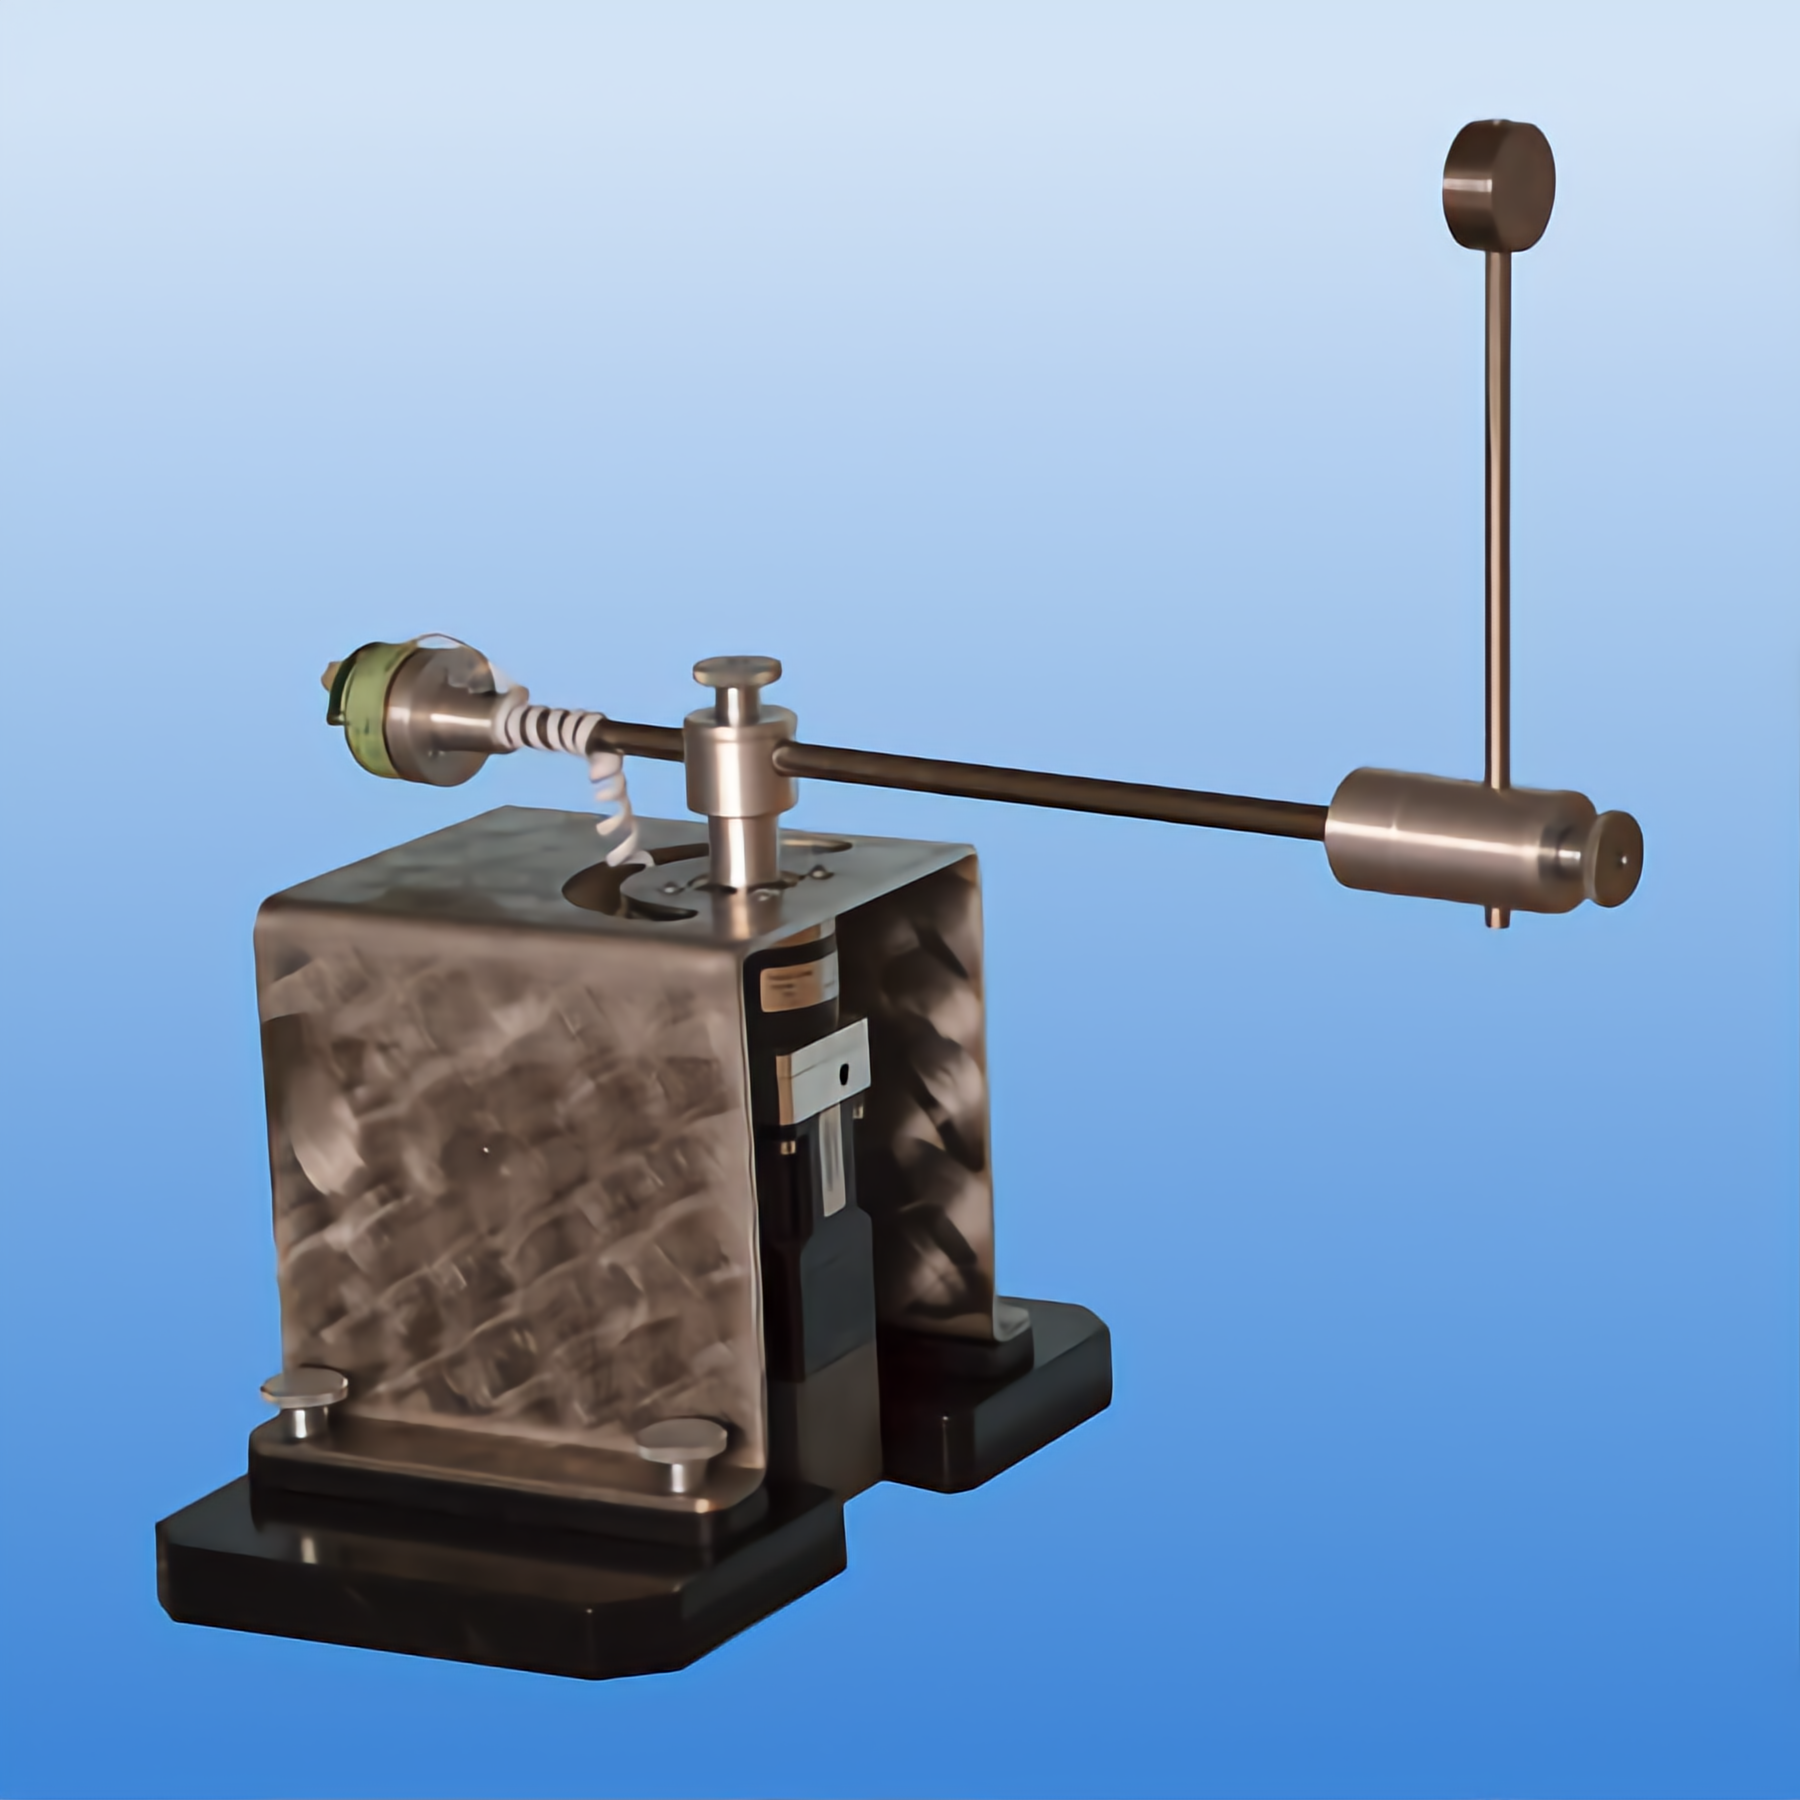
\includegraphics[width=.6\linewidth]{images/furutareal}
	\caption{Laboratory Furuta pendulum device}
	\label{furutareal}
\end{figure}
which values of parametres are given in the following table
\begin{table}[H]
	\caption{Values of Furuta Pendulum Parameters}

\begin{tabular}{l l l}	
	\noalign{\hrule height 1pt}
	Parameter&Symbol&Value\\
	\noalign{\hrule height 1pt}
	Gravitational acceleration&$g$&9.81\si{\metre\per\square\second}\\
	Mass of arm&$m_0$&0.6 \si{\kilogram}\\
	Mass of pendulum&$m_1$&0.198 \si{\kilogram}\\
	Length of arm&$L_0$&0.51 \si{\metre}\\
	Llength of pendulum&$L_1$&0.23 \si{\metre}\\
	Location of the pendulums center of mass&$l_1$&0.21 \si{\metre}\\
	Moment of inertia of arm&$I_0$&0.052 \si{\kilogram\per\square\metre}\\
	Moment of inertia of pendulum&$I_1$&8.72e-4 \si{\kilogram\per\square\metre}\\
	Sampling time&$T_s$&0.02 \si{\second}\\
	\hline
\end{tabular}
\label{furuta:values}
\end{table}
By substituting values from table \ref{furuta:values} into \ref{linSSmodel:general} and evaluating it at the upright operation point 
\begin{equation}
\ui{x}{up} = \begin{bmatrix}0,0,0,0\end{bmatrix}^\intercal, 
\end{equation}
the linear, continuouss-time State-Space model, representing the dynamic of the pendulum near the upright position is obtained
\begin{subequations}\label{linSSmodel:up}
	\begin{align}
	\ui{A}{c,up} &=\begin{bmatrix}
	0&1&\ 0& 0\\
	0&0&-15.8833&0\\
	0&0&\ 0&1\\
	0&0&\ \; \,77.5373&0
	\end{bmatrix},\\
	\ui{B}{c,up} &=\begin{bmatrix}
	\ 0\\
	\ \; \,17.6366\\
	\ 0\\
	-38.9393
	\end{bmatrix}.
	\end{align}
\end{subequations}
And with this model obtained, we are ready to proceed to controller design and pendulum control.
 
First a linear MPC strategy to stabilize the pendulum at the upright pozition will be designed. Second is the Energy-Shaping controller to swing the pendulum from the downside position. Then the MPC and Swing-Up controllers will be combined to perform Heuristic Swing-Up control of the pendulum. And finally via using a NMPC strategy an Optimal Swing-Up control of the pendulum will be performed.
\section{Model Predictive Controller}
Due to the pendulums setup, the MPC formulation (\ref{mpcgeneral}) could be applied directly. As known, a linear MPC uses a linear prediction model \ref{linSSmodel:up} of the process to predict the behavior of the system over the prediction horizon. Such a predictive model is only relevant in vicinity of linearization point. That is the reason why the linear MPC strategy is used to conrol the pendulum only around upright position. 
The MPC is a discrete-time strategy, therefore the first step of the construction of such a controller is to obtain the discrete-time linear predictive model. Such model can be derived from continuous-time model (\ref{linSSmodel:up}) by some discretization method. In this thesis a zero-order hold method, with the discretization step, equal to devices sampling time, $0.02 s$ is used. 
\begin{subequations}\label{dismatrices}
	\begin{align}
	\ui{A}{d} &=\begin{bmatrix}
	1&0.02&-0.0032& 0\\
	0&1&-0.3193&-0.0032\\
	0&0&\ \; \,1.0155&\ \; \,0.0201\\
	0&0&\ \; \,1.5588&\ \; \,1.0155
	\end{bmatrix},\\
	\ui{B}{d} &=\begin{bmatrix}
	\ \; \,0.0035\\
	\ \; \,0.3536\\
	-0.0078\\
	-0.7828
	\end{bmatrix}.\\
	\end{align}
\end{subequations}
The output matrices remain unchanged from (\ref{linmatrices}).\\ 

Now it is important to determine the range around the linearization point, where such a model is relevant. For that purpose will be evaluated the difference in outputs from the non-linear and linear model. For that purpose both models will be simulated with the same value of control input.
\begin{table}[H]
	\caption{Comparisson of linear and non-linear models}
	\label{models:comparisson}
\begin{tabular}{c c}	
	\noalign{\hrule height 1pt}
	Initial angle of the pendulum [deg]&Difference in outputs [deg]\\
	\noalign{\hrule height 1pt}
	30&0.5977\\
	40&0.8370\\
	50&1.0200\\
	60&1.1474\\
	70&1.2314\\
	\hline
\end{tabular}
\end{table}
Those results demonstrate that an MPC can be used to control the pendulum roughly in $\pm50deg$ around the upright position. Also, those results were obtained for the limit value of control input, for a smaller value of control input the difference, naturally, will be lesser.\\

The next, probably the most important, step is to design weight matrices $\ui{Q}{x}$ and $\ui{Q}{u}$. The main weights must be given to the position of the pendulum, what is our main controlled parameter, and the position of the arm, to prevent the possible scenario when the pendulum is stabilized at the upright position and the arm rotates constantly. 
\begin{equation}
\ui{Q}{x} = \begin{bmatrix}
1.5&0&0&0\\
0&0.08&0&0\\
0&0&10&0\\
0&0&0&0.2
\end{bmatrix}, \quad \ui{Q}{u} = 1.
\end{equation}
Weight matrices are the key point of MPC, as through them we define for MPC a requested control performance.
The remain MPC parametres can be set as shown in the following table
\begin{table}[H]
	\caption{MPC parameters during the stabilization at the upright position}
	\begin{tabular}{l c c}
		\noalign{\hrule height 1pt}
		Parameter&Symbol&Value\\
		\noalign{\hrule height 1pt}
		Prediction horizon&$N$&$20$\\
		Initial condition&$x_0$&$\begin{bmatrix}-1,-2,0.5,2\end{bmatrix}^\intercal$\\
		Constraint on control input-upper bound&$\ui{u}{max}$&$\ \; \,10$\\
		Constraint on control input-lower bound&$\ui{u}{min}$&$-10$\\
		\hline
	\end{tabular}
\end{table}
Due to the fact, that the Furuta pendulum performs a rotary motion, the safety constraints on the states are not necessary. So only present inequality constraints are the limit constraints on the control input.\\

Considering all aforesaid, the MPC formulation can be written in the following form
\begin{subequations}\label{mpc:linear}
	\begin{align}
	\min_{U}\ &\sum_{k=0}^{N-1} \lrp{\left\| \ui{Q}{x}x_{k}\right\|_2+\left\|\ui{Q}{u}u_{k}\right\|_2}\\
	\text{s.t.}\ &x_{k+1} = A_dx_{k} + B_du_{k}\qquad\qquad\ \ \,  k \in \mathbb{N}_0^{N-1}\\
	&x_0 = x(0)\\
	&\ui{u}{min}\leq u_{k}\leq \ui{u}{max}\qquad\qquad\qquad\;   k \in \mathbb{N}_0^{N-1}
	\end{align}
\end{subequations}
This predictive controller is designed in \textsc{MATLAB}, using the \textsc{YALMIP} toolbox \cite{YALMIP} to formulate the problem and \textsc{Gurobi} solver to solve it.
\newpage
\begin{figure}[H]
	\centering
	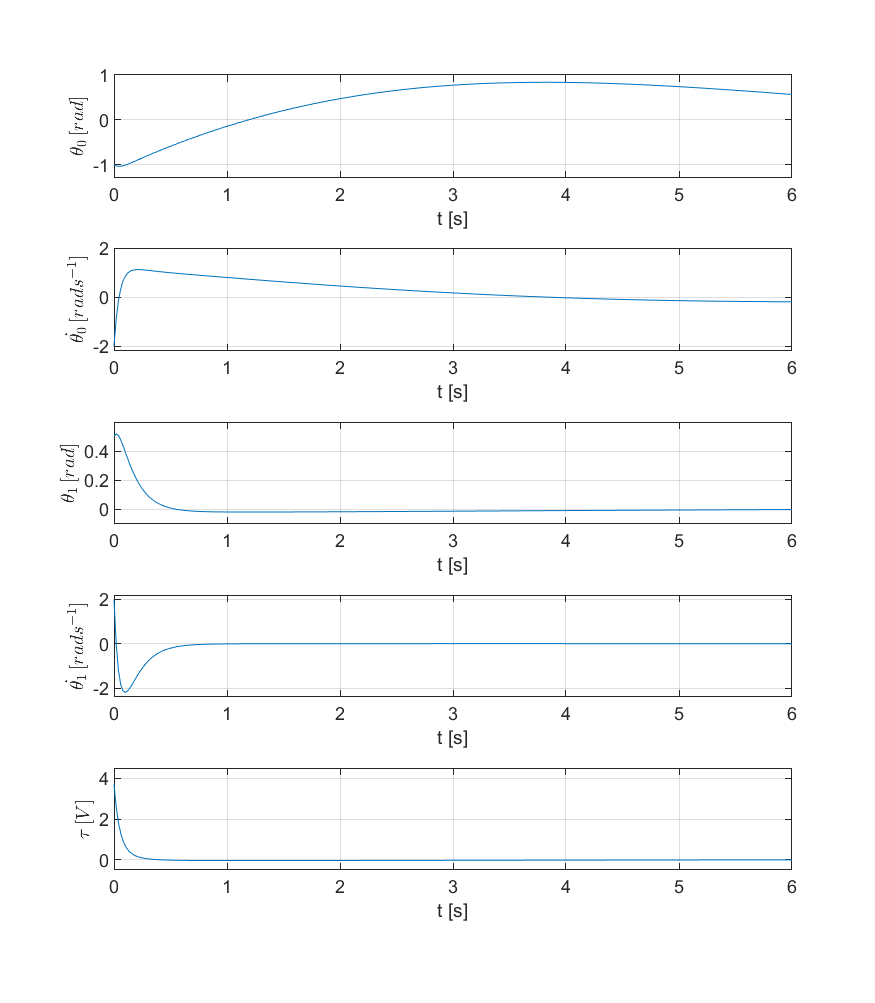
\includegraphics[width=1.1\linewidth]{images/MPC}
	\caption{Simulation results for a scenario with stabilization at the upright position by linear MPC. The plots depict, respectively, the individual states , the third of which is the controlled pendulum position $\theta_1(t)$, and the control input $\tau(t)$.}
	\label{mpc}
\end{figure}
The simulation results of stabilizing the pendulum at the upright position, using a linear MPC are shown in Fig.\ref{mpc}. As can be observed, such a predictive controller is capable of stabilizing the pendulum, without constraints violation. The only issue is the solving time. For this scenario, the solving time was $[0.0156, 0.0313]s$, which is not satisfying because of sample time. One possible solution is the hardware upgrade, as the simulations were performed on a rather old laptop.

\section{Energy-Shaping Controller}
The main purpose of the Energy-Shaping controller is to swing the pendulum from the downside position into the upright position where the control of the process will be taken by another controller. 
Such controller can be designed by applying the control law (\ref{energy-shaping}) directly as a state-feedback controller.
\newpage
\begin{figure}[H]
	\centering
	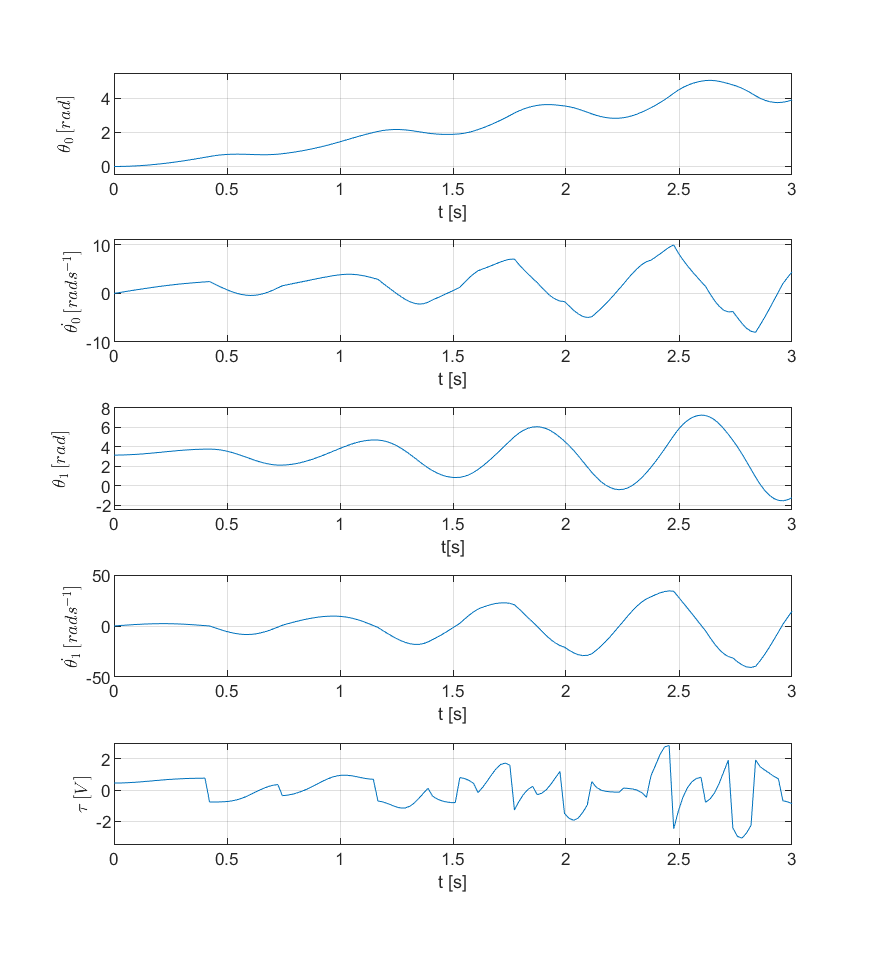
\includegraphics[width=1.1\linewidth]{images/Swing}
	\caption{Initial oscillation of the system by the Energy-Shaping controller. The plots depict, respectively, the individual states , the third of which is the controlled pendulum position $\theta_1(t)$, and the control input $\tau(t)$.}
	\label{swing}
\end{figure}
\newpage
\section{Heuristic Swing-Up Control}
To perform Swing-Up Control of the pendulum, a combined control strategy should be designed, because no MPC nor Swing-Up controller can not perform a Swing-Up control by itself. So the strategy of Heuristic Swing-Up Control is that at the beginning the pendulum is steady at the downside position and the Energy-Shaping controller is used to add the energy to the pendulum via its oscillation. As more energy is added to the pendulum, the greater the oscillations become. As the pendulum is close to the upright operation point, the control law switches from Energy-Shaping to MPC. And MPC finishes the Swing-Up Control by stabilizing the pendulum at the upright position.
\begin{figure}[H]
	\centering
	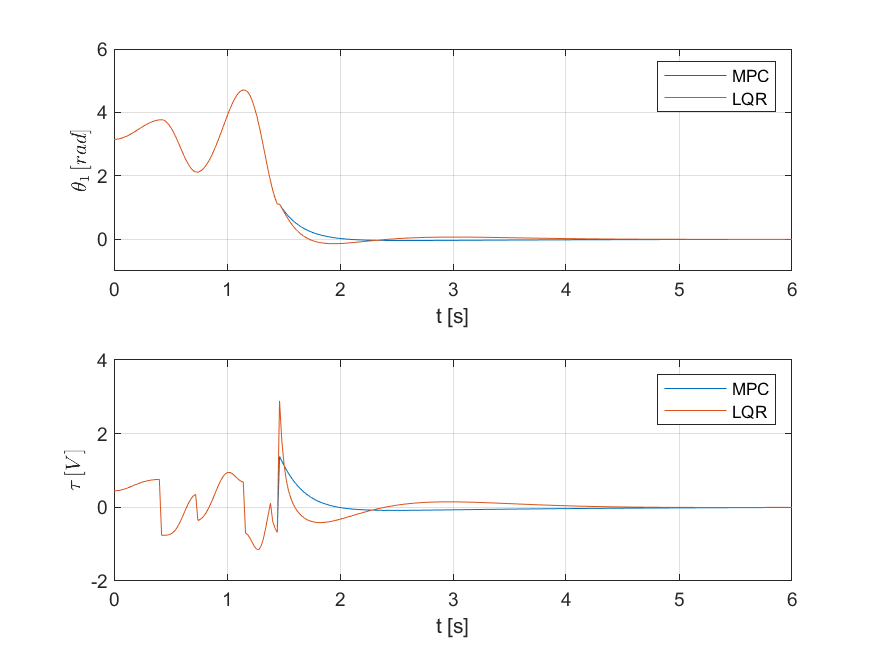
\includegraphics[width=1.1\linewidth]{images/MPC-LQR_Swing}
	\caption{Simulation result of the Swing-up control of the pendulum by Energy-Shaping+Mpc combined control strategy. The first plot depict the controlled pendulum position $\theta_1(t)$, and the second - control input $\tau(t)$.}
	\label{combo}
\end{figure}
\newpage
\section{Optimal Swing-Up Control}
The last control strategy is an Optimal Swing-Up Control. In this strategy, only one non-linear Model Predictive Controller (NMPC) is used to perform both the swing-up and the stabilization of the pendulum. Such control performance is possible due to the fact that in NMPC the non-linear model (\ref{nonlinmodel}) is used to predict the future evolution of the process.  Usage of this non-linear model, leads to a Non-linear Programing (NLP) problem, and solving a NLP problem is ot a trivial process. In this work a \textsc{MATMPC} toolbox is used \cite{MATMPC} to formulate and solve this problem.\\

 In general a NMPC problen can be formulated in similar form as linear MPC problem (\ref{mpc:linear}):
\begin{subequations}\label{nmpcgeneral}
	\begin{align}
	\min_{U}\ &\sum_{k=0}^{N-1} \lrp{\left\| \ui{Q}{x}x_{k}\right\|_2+\left\|\ui{Q}{u}u_{k}\right\|_2}\\
\text{s.t.}\ &x_{k+1} = f(x_{k}, u_{k})\qquad\qquad\qquad \ \   k \in \mathbb{N}_0^{N-1}\\
&x_0 = x(0)\\
&\ui{u}{min}\leq u_{k}\leq \ui{u}{max}\qquad\qquad\qquad\;   k \in \mathbb{N}_0^{N-1}
	\end{align}
\end{subequations}
The rules for weight matrices in NMPC strategy are similar to those, used in linear MPC strategy, except that to the arm is given more freedom and we are willing to invest more into control inputs. It's because of that the controller must not only stabilize the pendulum but also perform a swing-up.
\begin{equation}\label{NMPC:weights}
\ui{Q}{x} = \begin{bmatrix}
1&0&0&0\\
0&0.1&0&0\\
0&0&3&0\\
0&0&0&0.1
\end{bmatrix}, \quad \ui{Q}{u} = 0.1.
\end{equation}
Other NMPC parameters are shown in the following table
\begin{table}[H]
	\caption{NMPC parameters for the Optimal Swing-Up Control strategy}
	\begin{tabular}{l c c}
		\noalign{\hrule height 1pt}
		Parameter&Symbol&Value\\
		\noalign{\hrule height 1pt}
		Prediction horizon&$N$&$20$\\
		Initial condition&$x_0$&$\begin{bmatrix}0,0,\pi,0\end{bmatrix}^\intercal$\\
		Constraint on control input-upper bound&$\ui{u}{max}$&$\ \; \,10$\\
		Constraint on control input-lower bound&$\ui{u}{min}$&$-10$\\
		\hline
	\end{tabular}
\end{table}
The parameters are similar, that were used in MPC, except for the initial condition, that in case of NMPC the pendulum's steady downside position.\\

From a user perspective, the design of such an NMPC strategy, using \textsc{MATMPC} toolbox is trivial. You only have to set the NMPC parameters and define a prediction model (\ref{nonlinmodel}). And toolbox will automatically construct and solve the following NLP problem
\begin{subequations}\label{NLP}
	\begin{align}
	\min_{X,U}\ \frac{1}{2}&\sum_{k=0}^{N-1} (\left\| h_k(x_k, u_k)\right\|_2\ui{Q}{k}) + \frac{1}{2}\left\|h_N(x_N)\right\|_2\ui{Q}{N}\\
	\text{s.t.}\quad &x_{k+1} = \phi(x_{k},u_{k})\qquad\qquad\qquad\, k \in \mathbb{N}_0^{N-1}\\
	&x_0 = x(0)\\
	&\ui{u}{min}\leq u_{k}\leq \ui{u}{max}\qquad\qquad\qquad\;   k \in \mathbb{N}_0^{N-1}	
	\end{align}
\end{subequations}
where $h_k$ and $h_N$ are vector functions of state and control $(x, u)$, matrices $\ui{Q}{k}$ and $\ui{Q}{N}$ are the weights for each term for stage $k$. Matrix $\ui{Q}{k}$ have the size of $n_x+n_u\times N$ and matrix $\ui{Q}{N}$ have the size of $n_x\times 1$, where $n_x$ is a number of states and $n_u$ is the number of control inputs. Considering these rules and NMPC weight matrices (\ref{NMPC:weights}), the NLP matrices can be designed as
\begin{equation}\label{NLP:weights}
\ui{Q}{k} = \begin{bmatrix}
				1.0&\cdots&1.0\\
				0.1&\cdots&0.1\\
				3.0&\cdots&3.0\\
				0.1&\cdots&0.1\\
				0.1&\cdots&0.1
			\end{bmatrix}, \quad 
\ui{Q}{N} =	\begin{bmatrix}
				1.0\\
				0.1\\
				3.0\\
				0.1
			\end{bmatrix}.
\end{equation}
$\phi(x_{k},u_{k})$ is a numerical integration operator that solves the following initial value problem (IVP) and returns the solution at $t_{k+1}$.
\begin{equation}
0=\ui{f}{impl}\lrp{\dot{x}(t), x(t),u(t),t},\quad x(0)=x_k.
\end{equation}
In the next step, the listed above NLP problem is solved by the Sequential Quadratic Programming (SQP) method, which was described in the corresponding part of the thesis - Section \ref{SQP:theory}. Also, additional software must be installed:
\begin{itemize}
	\item \textbf{CasAdi} - to obtain the needed derivatives to perform optimization (\url{https://github.com/casadi/casadi/wiki}).
	\item \textbf{MinGW-w64 C/C++ Compiler} - to compile \textsc{MATMPC} modules into MEX functions with performance comparable to plain C/C++ solvers.
\end{itemize}
And with such setup, a Optimal Swing-Up control of the Pendulum can be performed
\newpage
\begin{figure}[H]
	\centering
	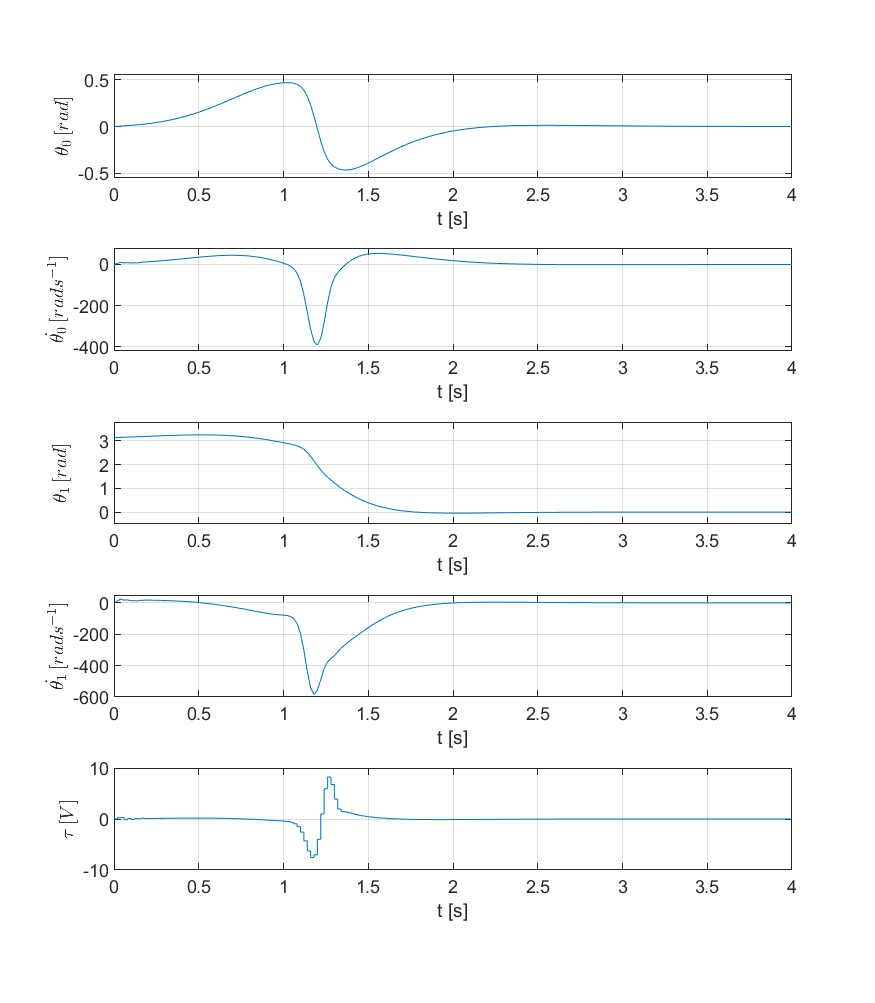
\includegraphics[width=1.1\linewidth]{images/NMPC}
	\caption{Simulation result of the Swing-up control of the pendulum by NMPC strategy.The plots depict, respectively, the individual states , the third of which is the controlled pendulum position $\theta_1(t)$, and the control input $\tau(t)$.}
	\label{NMPC:results}
\end{figure}
Considering the results in Fig.\ref{NMPC:results} we can conclude, that a non-linear predictive controller was designed correctly. It's capable to perform the Swing-Up control of the pendulum with its stabilization at the upright position without constraints violation. Also, the control was performed in an impressive time of $2.5\si{\second}$.